%%%%%%%%%%%%%%%%%%%% author.tex %%%%%%%%%%%%%%%%%%%%%%%%%%%%%%%%%%%
%
% sample root file for your "contribution" to a contributed volume
%
% Use this file as a template for your own input.
%
%%%%%%%%%%%%%%%% Springer %%%%%%%%%%%%%%%%%%%%%%%%%%%%%%%%%%


% RECOMMENDED %%%%%%%%%%%%%%%%%%%%%%%%%%%%%%%%%%%%%%%%%%%%%%%%%%%
\documentclass[graybox]{svmult}

% choose options for [] as required from the list
% in the Reference Guide

\usepackage{mathptmx}       % selects Times Roman as basic font
\usepackage{helvet}         % selects Helvetica as sans-serif font
\usepackage{courier}        % selects Courier as typewriter font
\usepackage{type1cm}        % activate if the above 3 fonts are
                            % not available on your system
%
\usepackage{makeidx}         % allows index generation
\usepackage{graphicx}        % standard LaTeX graphics tool
                             % when including figure files
\usepackage{multicol}        % used for the two-column index
\usepackage[bottom]{footmisc}% places footnotes at page bottom
 \usepackage{epstopdf}
 \usepackage{amssymb}
\usepackage{amsmath}
\usepackage{amsbsy}
\usepackage{wrapfig}
\usepackage{changebar}
\usepackage{xcolor}
\usepackage{rotating}
\usepackage[ruled,linesnumbered,vlined]{algorithm2e}
\usepackage[normalem]{ulem}
%% editing comment

%\newcommand{\cmt}[1]{\textcolor{red}{\textbf {#1}}}
\newcommand{\cmt}[1]{}
%\newcommand{\note}[1]{\cmt{Note: #1}}
\newcommand{\karen}[1]{\textcolor{red}{{Karen: #1}}}
\newcommand{\original}[1]{\textcolor{blue}{{Original: #1}}}
\newcommand{\del}[1]{\ignorethis{#1}}
\newcommand{\newtext}[1]{{#1}}
%\newcommand{\newtext}[1]{\textcolor{blue}{#1}}
\newcommand{\eqnref}[1]{Equation~(\ref{eqn:#1})}

%% ignore text
\long\def\ignorethis#1{}

%% abbreviations
\newcommand{\etal}{{\em{et~al.}\ }}
\newcommand{\eg}{e.g.\ }
\newcommand{\ie}{i.e.\ }

%% reference shortcuts
\newcommand{\figtodo}[1]{\framebox[0.8\columnwidth]{\rule{0pt}{1in}#1}}
\newcommand{\figref}[1]{Figure~\ref{fig:#1}}
%\renewcommand{\eqref}[1]{Equation~(\ref{eq:#1})}
\newcommand{\secref}[1]{Section~\ref{sec:#1}}

%% frequently used mathematical structures
\newcommand{\vc}[1]{\ensuremath{\mathbf{#1}}}
\newcommand{\pd}[2]{\ensuremath{\frac{\partial{#1}}{\partial{#2}}}}
\newcommand{\pdd}[3]{\ensuremath{\frac{\partial^2{#1}}{\partial{#2}\,\partial{#3}}}}


% math macros
\newcommand{\vEndEff}{\ensuremath{\vc{d}}}
\newcommand{\vRelMove}{\ensuremath{\vc{r}}}
\newcommand{\sSet}{\ensuremath{S}}


\newcommand{\vControl}{\ensuremath{\vc{u}}}
\newcommand{\vPoint}{\ensuremath{\vc{p}}}
\newcommand{\sSpringCoef}{{\ensuremath{k_{s}}}}
\newcommand{\sDamperCoef}{{\ensuremath{k_{d}}}}
\newcommand{\vHandle}{\ensuremath{\vc{h}}}
\newcommand{\vForce}{\ensuremath{\vc{f}}}

\newcommand{\mTransChain}{\ensuremath{\vc{W}}}
\newcommand{\mRotateTrans}{\ensuremath{\vc{R}}}
\newcommand{\sJoint}{\ensuremath{q}}
\newcommand{\vJoint}{\ensuremath{\vc{q}}}
\newcommand{\mJoint}{\ensuremath{\vc{Q}}}
\newcommand{\mMass}{\ensuremath{\vc{M}}}
\newcommand{\sMass}{\ensuremath{{m}}}
\newcommand{\vGravity}{\ensuremath{\vc{g}}}
\newcommand{\vConstr}{\ensuremath{\vc{C}}}
\newcommand{\sConstr}{\ensuremath{C}}
\newcommand{\vCOM}{\ensuremath{\vc{x}}}
\newcommand{\sGeneralForce}[1]{\ensuremath{Q_{#1}}}
\newcommand{\vStateVar}{\ensuremath{\vc{y}}}
\newcommand{\vControlVar}{\ensuremath{\vc{u}}}
\newcommand{\argmax}{\operatornamewithlimits{argmax}}
\newcommand{\tr}[1]{\ensuremath{\mathrm{tr}\left(#1\right)}}




%%%%%%%%%%%%%%%%%%%%%%%%%%%%%%%%%%%%%%%%%%%%%%%%%%%%%%%%%%%%%%%%%%%
%
% Here are a bunch of macros, mostly for math.
%
%%%%%%%%%%%%%%%%%%%%%%%%%%%%%%%%%%%%%%%%%%%%%%%%%%%%%%%%%%%%%%%%%%%

\renewcommand{\choose}[2]{\ensuremath{\left(\begin{array}{c} #1 \\ #2 \end{array} \right )}}

\newcommand{\gauss}[3]{\ensuremath{\mathcal{N}(#1 | #2 ; #3)}}

\newcommand{\pctab}{\hspace{0.2in}}
\newenvironment{pseudocode} {\begin{center} \begin{minipage}{\textwidth}
                             \normalsize \vspace{-2\baselineskip} \begin{tabbing}
                             \pctab \= \pctab \= \pctab \= \pctab \=
                             \pctab \= \pctab \= \pctab \= \pctab \= \\}
                            {\end{tabbing} \vspace{-2\baselineskip}
                             \end{minipage} \end{center}}
\newenvironment{items}      {\begin{list}{$\bullet$}
                              {\setlength{\partopsep}{\parskip}
                                \setlength{\parsep}{\parskip}
                                \setlength{\topsep}{0pt}
                                \setlength{\itemsep}{0pt}
                                \settowidth{\labelwidth}{$\bullet$}
                                \setlength{\labelsep}{1ex}
                                \setlength{\leftmargin}{\labelwidth}
                                \addtolength{\leftmargin}{\labelsep}
                                }
                              }
                            {\end{list}}
\newcommand{\newfun}[3]{\noindent\vspace{0pt}\fbox{\begin{minipage}{3.3truein}\vspace{#1}~ {#3}~\vspace{12pt}\end{minipage}}\vspace{#2}}



\newcommand{\key}{\textbf}
\newcommand{\fun}{\textsc}

%\def\shortcite{\def\citename##1{}\@internalcite}


% Local Variables:
% TeX-master: "paper"
% End:

%\DeclareMathOperator{\sgn}{sgn}


% see the list of further useful packages
% in the Reference Guide

\makeindex             % used for the subject index
                       % please use the style svind.ist with
                       % your makeindex program

%%%%%%%%%%%%%%%%%%%%%%%%%%%%%%%%%%%%%%%%%%%%%%%%%%%%%%%%%%%%%%%%%%%%%%%%%%%%%%%%%%%%%%%%%

\begin{document}

\title*{Physically-based Character Animation Synthesis}
% Use \titlerunning{Short Title} for an abbreviated version of
% your contribution title if the original one is too long
\author{Jie Tan}
% Use \authorrunning{Short Title} for an abbreviated version of
% your contribution title if the original one is too long
\institute{Jie Tan \at Georgia Intitute of Technology, Atlanta, Georgia, USA \email{jtan34@gatech.edu}}
%
% Use the package "url.sty" to avoid
% problems with special characters
% used in your e-mail or web address
%
\maketitle
\abstract{Understanding and synthesizing human motions is an important scientific quest. It also has broad applications in computer animation. Research on physically-based character animation in last two decades has achieved impressive advancement. A large variety of human activities are synthesized automatically in a physically simulated environment. The two key components of physically-based character animation are 1) physical simulation that models the dynamics of humans and their environment, and 2) controller optimization that optimizes the character's motions in the simulation. This approach has an inherent realism because we all live in a world that obeys physical laws, and we evolved to survive in this physical environment. In this chapter, we will review the state of the art of physically-based character animation, introduce a few established methods in physical simulation and motor control, and discuss promising future directions.}

\begin{keywords}
Character animation, Physical simulation, Trajectory optimization, Reinforcement learning.
  \end{keywords}
\section{Introduction}

Mother Nature has created a diverse set of awe-inspiring motions in the animal kingdom: Birds can fly in the sky, fishes can swim in the water, geckos can crawl on vertical surfaces, and cats can reorient themselves in mid-air. Similarly, human's motions exhibit efficiency (locomotion), agility (Kung Fu), gracefulness (Ballet) and dexterity (hand manipulation). Studying these motions is not only a scientific quest that quenches our curiosity, but also an important step towards synthesizing them in a way that can fundamentally change our life. Character animation aims to faithfully synthesize these motions of humans and animals, and display them to an audience for the purpose of entertainment, story-telling and education. For example, in movies and games, we need to faithfully reproduce the motions of humans and animals on the screen. The synthesized motions need to appear realistic to give the audience an immersive experience. 

In the last few decades, we have seen tremendous advance in character animation. Some of the most breathtaking movies, such as Harry Potter, Avatar and Life of Pi, rely heavily on computer generated character animations. Nowadays, it is almost impossible for the audience to tell apart the computer-synthesized motions from the real footage. Behind these realistic animations lies countless hours of tedious manual work of highly-specialized experts. For example, to produce a 100-minute feature film at Pixar can take dozens of artists and engineers more than five years of development. In today's animation pipeline, the most popular techniques to synthesize motions are key frames or motion capture, both of which require artistic expertise and laborious manual work. Even worse, the knowledge and efforts that are put into one animation sequence are not necessarily generalizable to other motions. In my point of view, these are not efficient or principled ways of animation synthesis.

\textbf{A principled way to synthesize character animation is to study the fundamental factors that have shaped our motions.} Instead of focusing on the appearance of our motions, we need to dig deeper to understand why we move in the way that we are doing today. After understanding the root causes that have shaped our movements, we can then synthesize them naturally and automatically. Our motions are shaped through millions of years of optimization (evolution) in a world that obey physical laws. This insight has motivated a new paradigm of \emph{Physically-Based Character Animation}. The two key components of this paradigm are physical simulation and motion control. We first build a physical simulation to model the physical world and then perform optimization to control the motions of characters so that they can move purposefully, naturally and robustly in the simulated environment. 

Although we often take our motion for granted since we can perform them so effortlessly, physically-based character animation is a notoriously difficult problem because out motions involve sophisticated neuromuscular control, sensory information processing, motion planning, coordinated muscle activation, and complicated interactions between the body and its physical environment. Even though we are still far from fully understand the underlying physics and control mechanisms that govern our motions, nearly two decades of research in physically-based character animation have brought us new insights, effective methodologies and impressive results. With the new development of physical simulation and motion control, realistic animation, including walking, running, fighting and grasping emerge automatically. In addition, the research in this field has developed algorithms that allow virtual characters to recover balance from unexpected perturbations, to move in different styles, to navigate through rough terrains and to demonstrate highly skillful stunts. The purpose of this chapter is to review these advancements (Section 2), introduce some of the established algorithms (Section 3), and discuss promising future research directions (Section 4) in physically-based character animation.


\section{State of the art}

\begin{figure}[h]
  \centering
  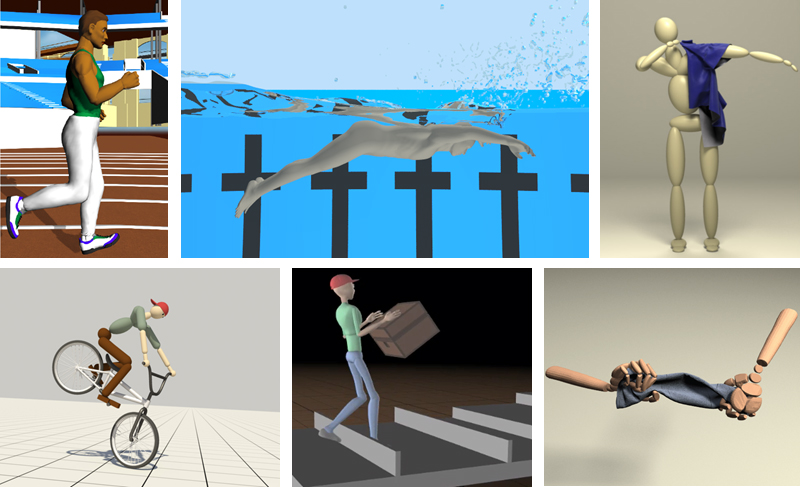
\includegraphics[width=\textwidth]{figures/teaser2.jpg}
  \caption{Variety of human activities, such as running, swimming, dressing, performing bicycle stunts, interacting with the environment and manipulating clothes, are simulated in a physically-simulated environment. Image courtesy \cite{Hodgins:1995:AHA,Si:2014,Clegg:2015,Tan:2014,Coros2010,Bai:2014}}
  \label{fig:teaser}
\end{figure}

Starting from the seminal work of Hodgins et al. \cite{Hodgins:1995:AHA}, controlling a physically simulated human character has been extensively studied in computer animation. A wide variety of human activities, including walking \cite{Yin:2007}, running \cite{Kwon:2010}, swimming \cite{kwatra2009fluid,Si:2014}, biking \cite{Tan:2014}, dressing \cite{Clegg:2015}, gymnastic motions \cite{Hodgins:1995:AHA}, reacting to perturbations \cite{Wang:2010}, falling and landing \cite{HA:2012:FLM} and manipulating objects with hands \cite{Liu:2009:DMF,Ye:2012,Bai:2014} are realistically synthesized in physically simulated environments (Figure \ref{fig:teaser}). 

Two main categories of methods to synthesize human motions are trajectory optimization and reinforcement learning. Trajectory optimization optimizes a motion trajectory by minimizing a task-related objective subject to physical constraints. It has been applied to control the iconic jumping Luxo Jr lamp \cite{Witkin:1988}, humanoid characters \cite{Liu:2002,Jain:2009,Ye:2010}, and characters with arbitrary morphologies \cite{Wampler:2009}. The resulting motions are physically plausible and follow the animation principles such as anticipation and follow-through \cite{thomas:1995}.  Reinforcement learning algorithms solve a Markov Decision Process (MDP) to find optimal actions at different states. If the transition model is known, (fitted) value iteration has been successfully applied to generalize motion capture data \cite{Treuille:2007:NCA,Levine:2012:CCC}, to carry out locomotion tasks \cite{Coros:2009:RTC}, and to manipulate objects with hands \cite{Multifinger2013}. Policy search \cite{Ng:2000:PPS} is another reinforcement learning algorithm that can directly searches for a control policy without the need to construct a value function. Many studies on locomotion control \cite{Yin08,Wang:2009,Coros:2011,Wang:2012,Geijtenbeek:2013} performed policy search on parameterized controllers. 

Although we have seen impressive advances for last two decades, the gracefulness, agility and versatility of real human motions remain unmatched. There are challenges in physically-based character animation that need further investigation. First, controlling balance is a key problem to synthesize human motions in a physically-simulated environment. Balance can be maintained by exerting virtual forces \cite{Pratt2001,Coros2010}, applying linear feedback \cite{Laszlo:1996,Yin:2007,daSilva:2008,Coros2010}, using nonlinear control policies \cite{Muico:2009}, planning the contact forces \cite{Muico:2009,Tan:2012}, employing reduced models \cite{Tsai:2010,Kwon:2010,Mordatch:2010:RPL,Coros2010,Ye:2010} and training in stochastic environments \cite{Wang:2010}. Although the balance problem in simple locomotion tasks, such as walking and running, has been solved, maintaining balance in tasks that require agile motions remains an open problem. 

Another challenge is to effectively plan the contacts. Humans move themselves and other objects through contacts. However, contact events (contact breakage, sliding, etc.) can introduce discontinuous forces to the dynamics equation, which breaks the control space into fragmented feasible regions. As a result, a small change in control parameters can easily generate bifurcated consequences. For this reason, many previous methods
explicitly assumed that the contacts remain static
\cite{Abe:2007,Jain:2009,Kim:2011:DCO} while optimizing control forces
subject to equations of motion. This assumption significantly
restricts the effectiveness of the controller for locomotion and balance
because the controller is not allowed to actively exploit contact
breakage, slipping contacts, or rolling contacts to achieve control
goals. Three promising research directions to tackle this challenge are contact-invariant optimization \cite{Mordatch:2012,Mordatch:2013}, solving QPCC \cite{Tan:2012} and policy search with stochastic optimization \cite{Wu:2010:TAB,Wang:2010,Mordatch:2010:RPL}.

An important criteria in physically-based character animation is the realism of the synthesized motions. Even today, the quality of motions synthesized in physically-based character animation is still far from natural. This has prevent it from be used for many applications. One possible cause of the unnatural motion is the vast simplification by representing the human character as an articulated rigid body system. To improve the realism, prior work has simulated the dynamics of muscles and demonstrated complex interplay among bones, muscles, ligaments and other soft tissues can be modeled for individual body parts, including
the neck \cite{Lee:2006}, the upper body \cite{Zordan:2006,Dilorenzo:2008,Lee:2009:CBM}, lower body \cite{Wang:2012}, and hands
\cite{Tsang:2005,Sueda:2008}. However, constructing such a sophisticated biological model for a full human character is still computational prohibitive. An alternative solution is to augment a physically controlled character with realstic motion capture streams \cite{daSilva:2008,Muico:2009:CAN,Liu:2010}. 















\section{Physical Simulation}

Physically-based character animation consists of two parts, simulation\index{simulation} and control\index{control}. This section concentrates on the simulation part while the next section on control. Although the majority of research in physically-based character animation focuses on control, a good understanding of physical simulation is essential for designing effective controllers because complex human behaviors often require sophisticated controllers that exploit the dynamics of a multi-body system.

\begin{figure}[h]
  \centering
  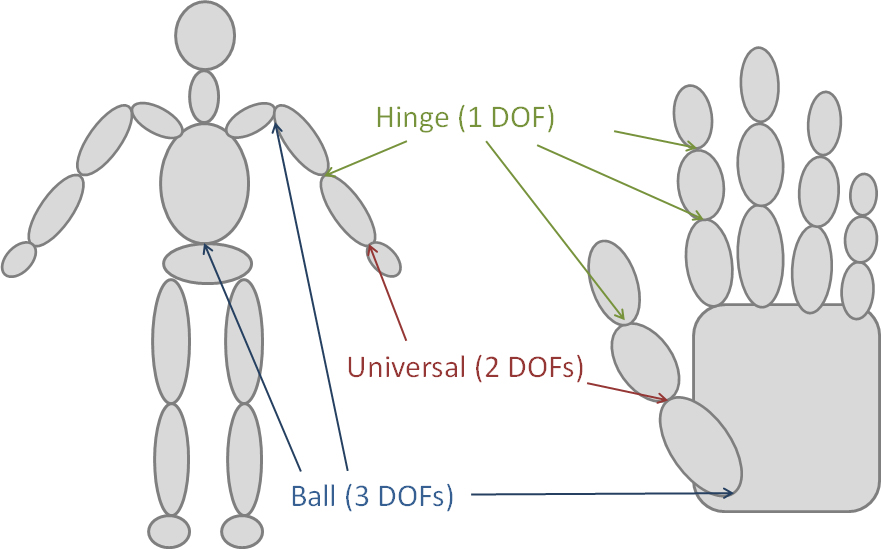
\includegraphics[width=0.6\textwidth]{figures/character.jpg}
  \caption{Articulated figures in character animation to represent a human character (left) and a hand (right).}
  \label{fig:character}
\end{figure}

In physically-based character animation, a human character is often represented as an articulated rigid body system\index{articulated rigid bodies} (Figure \ref{fig:character} left), a group of rigid bodies chained together through rotational joints\index{joint}. These joints can have different number of degrees of freedom (DOF)\index{DOF}. For example, the shoulder is a ball joint (3 DOFs), the wrist is a universal joint (2 DOFs) and the elbow is a hinge joint (1 DOF). In some cases, if the character's motion involves dexterous hand manipulation, a detailed hand model (Figure \ref{fig:character} right) is attached to each wrist. Note that the articulated rigid body system is a dramatic but necessary simplification since simulating each bone, muscle and tendon that a real human has would require a prohibitively huge amount of computational resources. In the simulation, the articulated figure is represented as a tree structure. Each node is a rigid body and each edge is a joint. One node can have multiple children but at most one parent. The root node has no parent. While any body can be selected as the root node, a common choice is to use the torso as the root. In this tree structure, loops are not allowed. Although it is possible to simulate loops, such case is rare in character animation and will not be discussed here. There are two major methods to simulate the dynamics of an articulated rigid body system: simulation in maximal coordinates\index{maximal coordinate} (Cartesian space)\index{Cartesian space} and simulation in generalized coordinates\index{generalized coordinate} (joint space)\index{joint space}.



\subsection{Simulation in Maximal Coordinates}
\index{maximal coordinate}
In maximal coordinates, the physical states of the articulated figures are defined for each node (rigid body). Each body has six degrees of freedom: three translational and three rotational. The dynamics of each rigid body is considered independently. A list of additional joint constraints \index{joint constraint}is imposed to ensure that the two adjacent bodies will stick together at the joint location. The dynamics equation \index{dynamics equation}for each body is 

\begin{equation}
\left[\begin{array}{cc}
m\vc{I}_{3\times3} & \vc{0} \\
\vc{0} & \vc{I}
\end{array}\right]
\left[\begin{array}{c}
\dot{\vc{v}} \\
\dot{\vc{\omega}}
\end{array}\right]=
\left[\begin{array}{c}
m\vc{g} \\
-\dot{\vc{I}}\vc{\omega}
\end{array}\right]
+\left[\begin{array}{c}
\vc{f}\\
\boldsymbol{\tau}
\end{array}\right]
+
\left[\begin{array}{c}
\vc{0}\\
\boldsymbol{\tau}^a
\end{array}\right]
\label{eq:dynamics}
\end{equation}
where $m$ and $\vc{I}$ are the mass and the inertia tensor of the body. $\vc{I}_{3\times 3}$ is a $3\times 3$ identity matrix. $\vc{v}$ and $\vc{\omega}$ are the linear and angular velocities. $[\vc{f}, \boldsymbol{\tau}]^T$ are the passive forces and torques from joint constraints, contacts, gravity and other external sources. $\boldsymbol{\tau}^a$ are the torques actively exerted by the controllers\index{controller}, which is the focus of Section 4.

Joints that connect two rigid bodies constrain their relative motions. Different number of constraints is imposed according to the type of joints. For example, a hinge joint has only one DOF. Thus it has five constraints that eliminate all but the rotation along the hinge axis. A ball joint has three DOFs. Its constraints eliminate the relative translation at the joint location. 

Suppose a joint connects body $A$ and body $B$, the translational constraints are:

\begin{displaymath}
\left[\begin{array}{c}
\vc{I}_{3\times 3}\\
-\vc{[r]}_{A\times}
\end{array}\right]
\left[\begin{array}{c}
\vc{v}_A \\
\vc{\omega}_A
\end{array}\right]-
\left[\begin{array}{c}
\vc{I}_{3\times 3}\\
-\vc{[r]}_{B\times}
\end{array}\right]
\left[\begin{array}{c}
\vc{v}_B \\
\vc{\omega}_B
\end{array}\right]
=\vc{0}
\end{displaymath}
where $[\vc{r}]_\times$ is the skew symmetric matrix of $\vc{r}$, which is the vector from the center of mass (COM) of the body to the joint location. The rotational constraints are:
\begin{displaymath}
\vc{d}_i^T(\vc{\omega}_A-\vc{\omega}_B)=0
  \end{displaymath}
where $\vc{d}_i$ is an axis perpendicular to the rotational DOFs and $i$ could be a subset of $\{0,1,2\}$ depending on the type of joints. 

To allow a character to actively control its motion, actuators are attached to the joints. According to Newton's third law, the two bodies connected to a common actuator should receive equal and opposite joint torques.
\begin{displaymath}
\boldsymbol{\tau}^a_A-\boldsymbol{\tau}^a_B=0
\label{eq:actuatorConstraint}
\end{displaymath}
where $\boldsymbol{\tau}_A$ and $\boldsymbol{\tau}_B$ are the torques exerted by the actuator to body $A$ and $B$ respectively.

Although simple to understand and implement, simulating characters in maximal coordinates has a few drawbacks. First, the state representation is redundant. It is not efficient to use all six DOFs of a rigid body and then eliminate most of them with joint constraints. Second, the accumulating numerical errors in simulation would cause the joint constraints not satisfied exactly. Eventually, joints will dislocate and adjacent bodies can drift apart. Both of these shortcomings can be overcome by simulation in generalized coordinates.

\subsection{Simulation in Generalized Coordinates}
\index{generalized coordinate}
In generalized coordinates, the physical states $\vc{q}, \vc{\dot{q}}$ of the articulated figure are defined on the edges of the tree (joint angles). Note that the root node is attached to the world space via a 6-DOF joint that can translate and rotate freely. Each DOF is one component of $\vc{q}$. The number of DOFs equals the dimensionality of $\vc{q}$. In other words, there is no redundancy in this representation.

The dynamics equation \index{dynamics equation}in generalized coordinates for an articulated rigid body system is:
\begin{equation}
  \vc{M}(\vc{q})\vc{\ddot{q}}+\vc{C(q,\dot{q})}=\vc{Q}+\boldsymbol{\tau}^a
  \label{eq:generalized}
\end{equation}
where $\vc{q}$, $\vc{\dot{q}}$ and $\vc{\ddot{q}}$ are the position, velocity and acceleration in generalized coordinates. $\vc{M(q)}$ is the mass matrix\index{mass matrix}. $\vc{C(q,\dot{q})}$ accounts for the Coriolis and centrifual force. $\vc{Q}$ is the external generalized force, including gravity and contact force. $\boldsymbol{\tau}^a$ is the generalized force exerted by the controller\index{controller} (Section 4). This equation can be derived from Lagrangian dynamics. Detailed derivation is omitted here but can be found in \citet{Liu:2012:STM}.

When the articulated rigid bodies are simulated in generalized coordinates, it is often necessary to convert physical quantities back and forth between generalized and maximal coordinates. For example, we need to compute the velocity at certain point on the articulated figure in Cartesian space for collision detection. We also need to convert the forces from the Cartesian space to generalized coordinates to apply contact forces. Jacobian matrix $\vc{J}$  bridges these two different coordinate systems.  
\begin{equation}
\vc{J}=\frac{\partial \vc{x}}{\partial \vc{q}}
\end{equation}
It represents the relation how much a point $\vc{x}$ moves in the Cartesian space if the joint angles $\vc{q}$ changes slightly. Here are the two most frequently-used formulas that convert velocities and forces, and more conversion formulas can be found in \citet{Liu:2012:STM}. 
\begin{displaymath}
  \begin{array}{lll}
    \vc{v} & = & \vc{J}\vc{\dot{q}}\\
    \vc{Q} & = &\vc{J}^T\vc{f}
   \end{array}
\end{displaymath}


Simulation in generalized coordinates is widely used in physically-based character animation. Although it takes more effort to walk through the derivation, it has important advantages over simulation in maximal coordinates. Apparently, the representation is more compact. There is no redundancy and thus no need to use constraints to eliminate redundant states. More importantly, it ensures that the joints are satisfied exactly. Two connecting bodies can never drift apart even with numerical errors because the states of dislocated joints are not part of the state space in generalized coordinates.

\subsection{Contact Modeling}
\index{contact}
Most of our daily activities, such as locomotion and hand manipulation, involve interacting with our surrounding environments through contacts. Accurately simulating contacts and computing contact forces are crucial to physically-based character animation. Penalty method\index{penalty method} and Linear Complementarity Problem (LCP)\index{LCP} are two widely used methods to model contact.

\subsubsection{Penalty Method}
\index{penalty method}
When a body $A$ penetrates another body $B$, a repulsive penalty force $\vc{f}_c$ is exerted to separate these two bodies.
\begin{equation}
\vc{f}_c=
\left\{
\begin{array}{cl}
-kd\vc{n} & \textrm{        if } d > 0,\\
0 & \textrm{        otherwise.}
\end{array}
\right.
\end{equation}
where $k$ is the stiffness, $d$ is the penetration depth and $\vc{n}$ is the contact normal. 

Penalty method is trivial to implement. However, to make it work properly, tedious manual tuning is often needed. While too small $k$ cannot effectively stop the penetration, too large $k$ would lead to undesired bouncy collision response. Even worse, when simulating with large time steps, penalty method could make the simulation unstable. In addition, it is not clear how to accurately model static friction using penalty methods.

\subsubsection{Linear Complementarity Problem}


\begin{figure}[h]
  \centering
  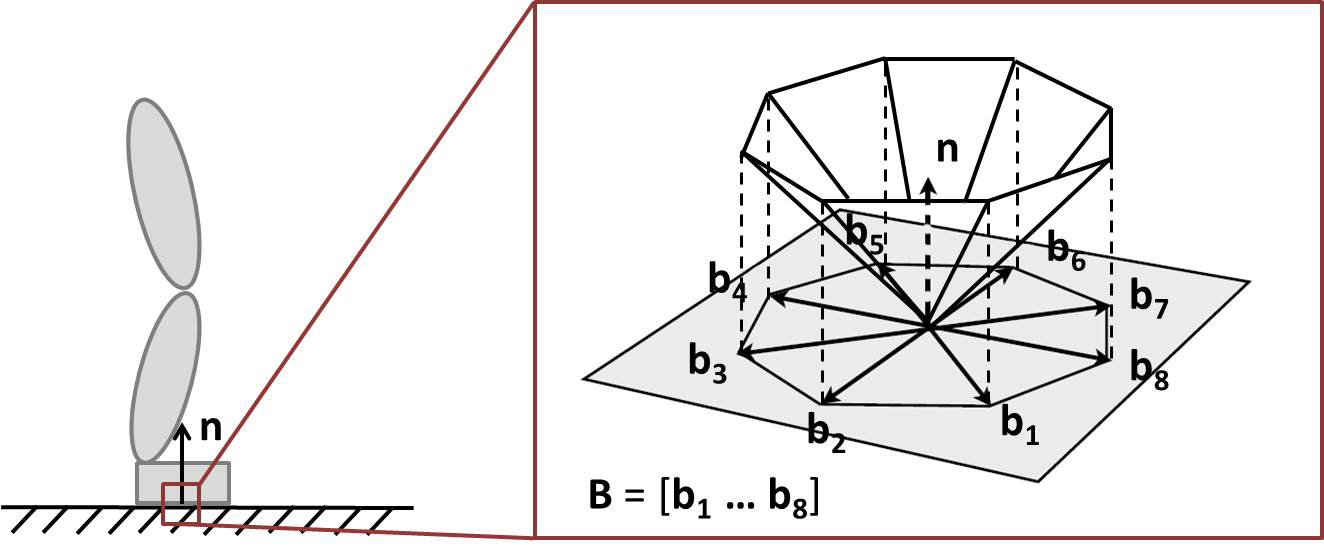
\includegraphics[width=0.85\textwidth]{figures/contact.jpg}
  \caption{A linearized friction cone used in LCP formulation. Left: a foot is in contact with the ground. Right: the friction cone at the contact point. $\vc{n}$ is the contact normal, and $\vc{b}_i$ are a set of tangential bases.}
  \label{fig:contactCone}
\end{figure}

Linear Complementarity Problem (LCP)\index{LCP} is a more accurate and stable method to model contacts. A contact force $\vc{f}_c$ can be decomposed into the normal and the tangential (frictional) forces.
\begin{displaymath}
\vc{f}_c = f_\perp\vc{n}+\vc{B}\vc{f}_{\parallel}
\end{displaymath}
where $\vc{n}$ is the contact normal, $f_\perp$ and $\vc{f}_{\parallel}$ are the normal and tangential components respectively. $\vc{B}$ is a set of bases that span the tangential plane (Figure ~\ref{fig:contactCone}). The more basis $\vc{b}_i$ are used, the more accurate approximation of the friction cone is, but more computation is needed to solve the resulting LCP. 

LCP imposes a set of constraints to satisfy the conditions of Coulomb friction: 1) In the normal direction, only repulsive forces are exerted to stop penetration. 2) In a static contact situation, the contact force lies within the friction cone. 3) In a sliding contact situation, the contact force lies at the boundary of the friction cone and the friction direction is opposite to the sliding direction. I will illustrate the concept of LCP using the formulation in the normal direction. The formulation in the tangential directions is beyond the scope of this chapter. It can be found in the following tutorials \cite{Lloyd:2005,Tan:2012b}. 

In a physical simulation, after the collisions are resolved, the relative velocity between the contact points of two colliding bodies can only be either zero (resting) or positive (separating), but not negative (penetrating):
\begin{equation}
v_\perp\geq 0
\label{eq:separating}
\end{equation}
Similarly, the normal contact force can be zero (no force) or positive (repulsive force), but not negative (sticking force):
\begin{equation}
f_\perp \geq 0
\label{eq:repulsive}
\end{equation}
The repulsive normal force exists ($f_\perp>0$) if and only if the two bodies are in contact ($v_\perp=0$). In contrast, when they are separating ($v_\perp>0$), there is no contact force ($f_\perp=0$).
In other words, the following linear complementarity condition\index{LCP} needs to be satisfied:
\begin{equation}
v_\perp f_\perp =0
\label{eq:complementarity}
\end{equation}

Combining the dynamics equations (eq. \ref{eq:dynamics} or ~\ref{eq:generalized}) and the LCP constraints (eq. \ref{eq:separating}, \ref{eq:repulsive}, \ref{eq:complementarity}) forms a mixed LCP problem. It can be solved efficiently by direct \cite{Lloyd:2005} or iterative solvers \cite{Erleben:2007,Kaufman:2008,Otaduy:2009}. 


\subsection{Simulation Software}

There is a growing need for simulation software that can accurately simulate the complex dynamics of virtural humans and their interactions with their surrounding environment. A number of open source physical simulators are readily available for research in physically-based character animation. The popular ones include Open Dynamic Engine (ODE) \footnote{http://www.ode.org/}, Bullet \footnote{http://www.bulletphysics.org/}, Dynamic Animation and Robotics Toolkit (DART) \footnote{http://dartsim.github.io/} and MuJoCo \footnote{http://www.mujoco.org}. All of them can simulate articulated rigid bodies\index{articulated rigid bodies} with an LCP-based\index{LCP} contact\index{contact} model in real time. These simulators allow the user to specify the structure of the articulated figure, the shape and the physical properties of each body, the type of joints, and other parameters describing the environment. Different simulators may offer different features, speed and accuracy. \citet{ErezTT15} provided an up-to-date review and an in-depth comparison among these modern physical engines.

\section{Motion Control}
\index{control}
We human can carefully plan our motion, coordinately and purposeful exercise our muscles to achieve high-level tasks, ranging from simple locomotion, dexterous hand manipulation, to highly skillful stunts. To model them in animation, simulating the passive dynamics is not enough. The key challenge that motion control tackles is to find controllers that can achieve these high-level motion tasks (e.g. walk at 1 m/s, grasp a bottle and open the cap, etc.). In character animation, a controller is the character's ``algorithmic brain'' that decides how much torque ($\boldsymbol{\tau}^a$ in eq. \ref{eq:dynamics} and \ref{eq:generalized}) are needed at each joint to successfully fulfill the task in a way that mimics human behavior. Motion control is the most extensively researched topic in physically-based character animation. Most methods use optimization. The optimizer searches for a controller that minimizes a task-related cost function, subject to dynamical constraints.

\begin{figure}[h]
  \centering
  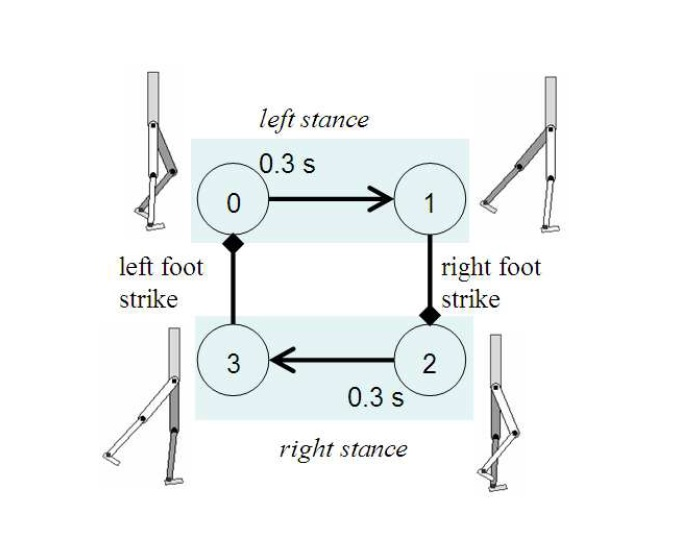
\includegraphics[width=0.55\textwidth]{figures/stateMachine.jpg}
  \caption{Different stages of walking used in SIMBICON. Image courtesy of \cite{Yin:2007:SIM}.}
  \label{fig:stateMachine}
\end{figure}

One common misunderstanding is that one can formulate a large optimization for arbitrary tasks. Due to complexity of human motions and nonlinearity of the dynamics, a large optimization may have competing objectives and many local minima. Up till today, there is no efficient optimization algorithms that can reliably find meaningful controllers in these cases. For this reason, a common practice in this field is to decompose a high-level task into multiple lower-level subtasks and formulate smaller optimization for each of the simpler subtask. For examples, In SIMBICON \cite{Yin:2007:SIM}, a walking cycle is decomposed into multiple stages (Figure \ref{fig:stateMachine}). Within each stage, separate optimizations can be used for controlling the two legs, the upper body, the balance and the style. After solving all the optimizations, these low-level controllers can be combined so that the character can walk naturally and robustly. Controller decomposition depends on the task and requires domain knowledge. We refer the readers to the research literature to learn controller decomposition on a case-by-case basis. In this section, we will discuss two generic optimization-based methods of motion control: trajectory optimization and reinforcement learning. 



\subsection{Trajectory Optimization}
\index{trajectory optimization}
Starting from the classical paper ``Spacetime Constraints''\index{spacetime constraints} \cite{Witkin:1988}, trajectory optimization has become a mainstream technique in physically-based character animation. It searches for a controller that minimizes a cost function subject to physical constraints. The general form of the optimization is:
\begin{equation}
  \begin{array}{cl}
    \min_{\vc{x},\vc{u}}&\sum_{t=0}^{N}g(\vc{x}_t,\vc{u}_t)\\
    \textrm{subject to}&\\
    &\vc{x}_{t+1}=\vc{h}(\vc{x}_t)+\vc{B}_t\vc{u}_t
  \end{array}
  \label{eq:trajectoryOptimization}
\end{equation}
where $\vc{x}$ is the physical states and $\vc{u}$ is the control. In character animation, the states are usually $\vc{x}=\vc{[q, \dot{q}]}^T$ and the control is $\vc{u}=\boldsymbol{\tau}^a$. $g$ is the cost function, which is often hand crafted to reflect the high-level task. For example, if the task is to walk at 1 m/s, one term in the cost function could be the distance between the current COM of the character and a desired COM position that moves at 1 m/s. The constraint usually consists of the dynamics equations $\vc{h}$. Note that in many applications of character animation, the dynamics are nonlinear to the state $\vc{x}$ but linear to the control $\vc{u}$ (See eq. \ref{eq:dynamics} and \ref{eq:generalized}). In addition, the constraints can also include joint limits, torque limits, and other task-related requirements.

To make it more concrete, we will revisit a simple example in the original ``Spacetime Constraints''\index{spacetime constraints} paper: controlling a single particle. The task of this particle is to fly from point $\vc{a}$ to point $\vc{b}$ in $T$ seconds using a time-varying jet force $\vc{f}(t)$. The dynamics of the particle is $m\vc{\ddot{x}}-\vc{f}-m\vc{g}=0$, where $\vc{x}$ is its position, $m$ is its mass and $\vc{g}$ is gravity. The goal of this flight is to minimize the total fuel consumption $\int_0^T|\vc{f}|^2dt$. After discretization along time, the optimization has the following form:
\begin{displaymath}
  \begin{array}{cl}
    \min_{\vc{x},\vc{f}}&\sum_{t=0}^{N}|\vc{f}_t|^2\\
    \textrm{subject to}&\\
    &\vc{x}_{t+1}= 2\vc{x}_{t} -\vc{x}_{t-1}+\frac{\Delta t^2}{m}\vc{f}_t+\Delta t^2\vc{g}\\
    &\vc{x}_0=\vc{a}\\
    &\vc{x}_N=\vc{b}
  \end{array}
  \end{displaymath}

It is not too difficult to extend the above derivations to control a human character. We will need to change the control force $\vc{f}(t)$ to joint torques $\boldsymbol{\tau}^a(t)$, the physical constraint to the dynamics equation of articulated rigid bodies (eq. \ref{eq:dynamics} or \ref{eq:generalized}), and the cost function to the relevant function specific to the task.

There are different options to solve the optimization according to the structure of the problem. Assuming the cost function and the dynamics equations are smooth, \citet{Witkin:1988} applied a generic nonlinear optimizer, Sequential Quadratic Program (SQP)\index{SQP}, to solve the problem. It is an iterative optimization technique that solves a sequence of quadratic programs that approximate the original problem. The solution of SQP is an optimal trajectory of state $\vc{x}^*(t)$ and control $\vc{u}^*(t)$. Note that this method produces a \emph{feedforward}\index{feedforward} (open-loop) controller: a trajectory over time. It cannot be generalized to the neighboring regions of the state space. As a result, the controller will fail the task even with a slight disturbance to the motion.

When the cost function is quadratic and the dynamics equation is linear,
\begin{equation}
  \begin{array}{cl}
    \min_{\vc{x},\vc{u}}&\sum_{t=0}^{N}\vc{x}_t^T\vc{Q}_t\vc{x}_t+\vc{u}_t^T\vc{R}_t\vc{u}_t\\
    \textrm{subject to}&\\
    &\vc{x}_{t+1}=\vc{A}_t\vc{x}_t+\vc{B}_t\vc{u}_t
  \end{array}
  \label{eq:LQR}
\end{equation}
the trajectory optimization is called an LQ problem. This problem can be solved very efficiently by linear-quadratic regulator (LQR)\index{LQR}. The derivation of LQR can be found in most of optimal control textbooks \cite{todorov2006optimal}. Thus we will not repeat it here. The solution is a \emph{feedback}\index{feedback} (close-loop) controller $\vc{u}_t=\vc{K}_t\vc{x}_t$. Although the requirement of linear dynamics seems quite restrictive, LQR still plays an important role in physically-based character animation. One important application is to design a physically-based controller to track motion captured data, which is an effective way to increase the realism of the synthesized motions. Given a motion capture\index{motion capture} sequence $\vc{\bar{x}}$, we can linearize the dynamics equation at its vicinity:
\begin{displaymath}
  \Delta \vc{x}_{t+1}=\frac{\partial \vc{h}}{\partial \vc{x}}\Delta \vc{x}_{t}+\vc{B}_t\vc{u}_t+\vc{h}(\vc{\bar{x}}_t)-\vc{\bar{x}}_{t+1}
  \end{displaymath}
where $\Delta \vc{x}=\vc{x}-\vc{\bar{x}}$. This gives an LQ problem that seeks a feedback\index{feedback} controller $\vc{u}_t=\vc{K}_t\Delta \vc{x}_t$ that minimizes the difference between the actual and the reference motion over the entire trajectory.

More importantly, LQR is a building block to solve the more general trajectory optimization problem (eq. \ref{eq:trajectoryOptimization}). Given an initial trajectory $\vc{x}_0, \vc{u}_0, \vc{x}_1, \vc{u}_1, ... , \vc{u}_N, \vc{x}_N$, we can perform the following steps iteratively:
\begin{enumerate}
\item{Compute the LQ approximation of the original problem (\ref{eq:trajectoryOptimization}) around the current trajectory by computing a first-order Taylor expansion of the dynamics, and a second-order expansion of the cost function.}
\item{Use LQR to solve the LQ approximation to get an optimal controller.}
\item{Apply the current optimal controller to generate a new trajectory.}
  \item{Go to Step 1 until convergence.}
\end{enumerate}
This iterative-LQR process\index{iterative-LQR} is similar to the core idea behind differential dynamic programming (DDP)\index{DDP}. We refer the interested reader to \citet{todorov2006optimal} for a more thorough discussion about LQR and DDP. The key advantage of DDP is that it not only provides a single trajectory, but also an optimal feedback controller near that trajectory.

To sum up, trajectory optimization is an effective way to synthesize character animation. The synthesized motion is not only physically correct, but more importantly, demonstrates an important animation principle, anticipation. This is because the objective of trajectory optimization is to minimize a long-term cost. Thus, the character can move intelligently that gives up short-term gains to minimize the long-term cost. For example, for a jump-up task, the trajectory optimization could produce a controller that sacrifices the height of the character's COM first for a much higher jump later. However, there are a few shortcomings of trajectory optimization. First, it often leads to a high dimensional optimization that is computational expensive to solve. Another problem of high dimensional nonlinear optimization is that the solver is more likely to get stuck at bad local minima. Thus, a good initialization is extremely important. Last but not least, trajectory optimization exploits the mathematical form of dynamic equations to design the optimal controller. If the dynamics is not smooth, too complicated or unknown, it is not clear how to apply trajectory optimization methods.


\subsection{Reinforcement Learning}
\index{reinforcement learning}
Reinforcement learning is motivated by the learning process of humans. In a high level, reinforcement learning optimizes a controller by interacting with the physical environment with numerous trials. Initially, the controller tries out random moves. If a desired behavior is observed, a reward is provided as the positive reinforcement. This reward system will gradually shape the controller until eventually it successfully fulfills the high-level task. Reinforcement learning is an active research area, with a large number of algorithms proposed every year. We refer readers to \cite{Kaelbling1996,Bagnell:2013} for a thorough review. We will focus on policy search\index{policy search} in remaining of this section. Policy search is a popular reinforcement learning algorithm in physically-based character animation. It performs extremely well in this field because it can tackle control problems with high-dimensional continuous state and action spaces, which is essential to control a human character. 

Mathematically, reinforcement learning solves a Markov Decision Process (MDP)\index{MDP}. An MDP is a tuple $(S, A, R, D, \gamma, P_{sas'})$, where $S$ is the \emph{state}\index{state} space; $A$ is the \emph{action}\index{action} space. The states reflect what the current situation is and the actions are what a character can perform to achieve the specified task. $R$ is the \emph{reward function}\index{reward function}. A reward function is a mapping from the state-action space to a real number: $R: S\times A\mapsto \mathbb{R}$, which evaluates how good the current state and action are. $D$ is the distribution of the initial state $s_0 \in D$ and $\gamma \in [0, 1]$ is the discount factor of the reward over time. $P_{sas'}$ is the \emph{transition probability}\index{transition probability}. It outputs the probability that the next state is $s'$ if an action $a$ is taken at the current state $s$. In physically-based character animation, the transition probability is computed by physical simulation. Although most of the physical simulations are deterministic, random noise can be added in simulation to increase the robustness of the learned controller \cite{Wang:2010}.

The solution of an MDP is a control \emph{policy}\index{policy} $\pi$ that maps the state space to the action space $\pi: S\mapsto A$. It decides what actions to take at different situations. Note that the goal of MDP is not to maximize the short-term reward $R$ at the next state, but a long term value function $V$. The \emph{return} of a policy is the accumulated rewards along the state trajectory starting at $s_0$ by following the policy $\pi$ for $N$ steps.
\begin{displaymath}
V^\pi(s_0)=\sum_{i=0}^N{\gamma^{N-i}R(s_i, \pi(s_i))}
\end{displaymath}
The reward at earlier states can be exponentially discounted over time. The \emph{value} of a policy is the expected return with respect to the random initial state $s_0$ drawn from D.
\begin{equation}
V(\pi)=E_{s_0\sim D}[V^\pi(s_0)]
\label{eq:policyValue}
\end{equation}
Using $V$ instead of $R$ as the optimization target prevents the controller from applying short-sighted greedy strategies. This agrees with our ability of long-term planning when we are executing our motions.

To formulate an MDP, we need to design the state space $S$, the action space $A$, the reward function $R$ for a given high-level task. Ideally, the state space should contain all the possible states of the articulated rigid body system, including the joint angles $\vc{q}$, joint velocities $\dot{\vc{q}}$ and time $t$, and the actions should include all the joint torques $\vc{\tau}^a$. However, this means that the state and the action space can have hundreds of dimensions. Due to the \emph{curse of dimensionality}, solving an MDP in such a high dimensional continuous space is computational infeasible. In practice, researchers often carefully design states and actions specifically for the tasks in question to make the computation tractable. For example, if the task is to keep balance while standing. The state space need only include important features for balance, such as the character's COM and the center of the ground contact polygon. Similarly, given the well-known balance strategies, such as ankle strategy and hip strategy, the action space can be as simple as a few torques at lower body joints. Using prior knowledge\index{prior knowledge} of the task can greatly simplify the problem, which is a common practice in physically-based character animation. 

A reward function for character animation usually consists of two parts, a task-related component that measures how far the current state is from the goal state and a component evaluates the naturalness of the motions. Designing a good reward function is essential to the success of the entire learning algorithm. A good design of the reward should be a smooth function that gives continuous positive reinforce whenever progress is made. Mathematically, this design will present gradient information that optimization solvers can follow. In contrast, a common mistake is to give reward only when the task is achieved, which makes the reward function a narrow spike and flat zero elsewhere. This should be avoided because nearly all the optimization algorithms would have trouble finding such a spike.

To apply policy search to solve the MDP, we need to parameterize the policy\index{policy parameterization}. A policy can be any arbitrary function. A practical way to optimize it is to parameterize it and then search for the optimal policy parameters. Commonly-used parameterizations include look-up tables, linear functions, splines and neural networks. Parameterization determines the potential quality of the final policy. However, there is no consensus what the best way is to parameterize a policy. It is decided on a case-by-case basis. Once the policy parameterization is decided, the initial policy is iteratively evaluated and improved until the optimization converges or a user-specified maximum number of iterations is reached.

To evaluate a policy\index{policy evaluation}, we can execute the policy in the simulation for N time steps with different initial states $s_0\in D$, accumulate the rewards and average the returns to compute the value of the policy. Policy improvement adjusts the policy parameters to increase its value. A straightforward way is to follow the policy gradient \cite{Ng:2000:PPS}. However, in many character animation tasks, such as locomotion and hand manipulation, contact events happen frequently, which introduces unsmooth contact forces that invalidates policy gradient. For this reason, sample-based stochastic optimization techniques are particularly suited for physically-based character animation. Covariance Matrix Adaptation Evolution Strategy (CMA-ES)\index{CMA-ES} \cite{hansen2006cma} is the most frequent applied optimization methods for motion control. CMA can work as long as we can evaluate the policy. It does not need to compute gradient and does not rely on good initializations. More importantly, CMA is a ``global'' search algorithm that explores multiple local minima. Although there is no guarantee that CMA will converge at the global minimum, in practice, it often finds good local minima in moderately high dimensional control spaces (\eg 20-30 dimensions). For the completeness of the chapter, we will briefly describe the CMA algorithm. Readers can refer to the original paper \cite{hansen2006cma} for additional details.

CMA starts with an initial underlying Gaussian distribution with large covariance in the policy parameter space. A population of samples is drawn from this distribution. The first generation of samples can be anywhere in the parameter space due to the large covariance matrix. Each CMA sample represents a control policy. The policies are evaluated through simulation. They are sorted according to their values and a certain percentage of the inferior samples are discarded. The underlying Gaussian distribution is updated according to the remaining good samples and is used to generate the next generation of the samples. This process is performed iteratively. Over iterations, the underlying distribution is shifted and narrowed. Eventually, the distribution converges to a good region of the policy space. The best CMA sample throughout all the iterations is selected as the optimal control policy.

In summary, reinforcement learning is a generic method for motion control. It can automatically learn a wide range of behaviors through simulation trials. Reinforcement learning, more specifically, policy search\index{policy search}, is becoming one of the most popular approaches in character animation synthesis. Reinforcement learning does not assume any mathematical forms of the dynamics equation. It treats the physical simulation as a black box, as long as it can output the next state given the current state and action. Thus, it is not bounded to a particular dynamics model. The same learning algorithm can still work even if the simulation software is upgraded. The main challenge of reinforcement learning is to design the states, the actions, the reward and the policy parameterization. We need to inject enough prior knowledge\index{prior knowledge} into the design so that the search space is small enough to be computationally feasible, but not too small that to contain effective policies. This requires a lot of experience and manual tweaking, especially for challenging motion tasks. 

\section{Conclusion and Future Directions}
\subsection{Conclusion}
In this dissertation, we have presented a principled way to synthesize locomotion of humans and animals. Our algorithms can control characters of different morphologies to move efficiently and robustly in complex physically-simulated environments and to achieve challenging tasks. The key components of our algorithms are a set of powerful computational tools, including physical simulation and controller optimization. Although combining simulation and optimization is not a novel idea in motion synthesis, in contrast to prior work, we examine and identify those commonly-used simplifications that can affect the quality of the motions. We eliminate these simplifications by designing new simulation and optimization techniques. Our simulators are faster, more stable and more accurate. Our optimizator can search a higher-dimensional space with both continuous and discrete variables, which may lead to better optimal solutions. These computational tools make it possible to study a more diverse set of motions in nature than were previous possible in the character animation literature.

Chapter 3 described computational tools to study the diversity of swimming motions for aquatic creatures with different body shapes. This is made possible by an accurate swimming simulation and a powerful evolutionary optimization. Compared to the simplified fluid model, our swimming simulation solves the Navier-Stokes equations. It can capture important features of water, including incompressibility and vortices, that affect swimming strategies. In contrast to the traditional alternating two-way coupling technique, our simulation solves the dynamic equations of fluids and articulated rigid bodies simultaneously. This increases the numerical stability and drastically speed up the computation. Simulating the hydrodynamic environment with Navier-Stokes equations introduce new challenges to the classical optimization algorithms. We demonstrated that CMA works well in this scenario. As a result, our algorithms can discover the most efficient swimming gait for a given creature automatically, without any human intervention. Our results showed that the synthesized swimming motions agree well with those employed by real aquatic animals.

Chapter 4 presented computational tools to study locomotion of soft body characters without skeleton support. We developed a muscle model that worked seamlessly with the state-of-the-art FEM simulation for soft materials. This muscle model is inspired by muscle structures found in real soft body animals. It lowers the dimensionality of the control space and ensures that the overall motion is coordinated. We demonstrated how to use finite-horizon trajectory optimization to control the locomotion. The key to our success is to identify that the widely-used simplification that separates contact planning with controller optimization is not good enough to achieve a stable locomotion. To solve this problem, we formulated a QPCC and developed an efficient solver. Consequently, effective control strategies and natural locomotion emerge automatically from the optimization solution.

Chapter 5 demonstrated computational tools to study agile human motions on a bicycle. We developed the first reinforcement learning algorithm that allows a virtual human character to learn bicycle stunts in a physically simulated environment. The algorithm is so efficient that most of stunt actions are learned in hours, which is even faster than the best human stunt bikers. An important lesson we have learned in this work is that it is difficult to design a good controller parametrization manually, especially for challenging locomotion tasks. The common practice of using a fixed policy parametrization tuned by users can severely limit the power of policy search algorithms. We eliminated this restriction by using NEAT, an algorithm that can simultaneously optimize both the parametrization and the parameters of a neural network. Eventually, the virtual character learned to perform a wide variety of stunts automatically, without the tedious manual tuning of controller parametrizations.

Chapter 6 explored an efficient method to develop humanoid robot controllers for the tasks of rising from a leaning/sitting/kneeling position to an erect stance. We built an accurate physical simulation, optimized controllers in the simulation and transferred the controller to a real robot. We investigated several factors that lead to the Reality Gap and demonstrated in several cases that this gap may be crossed with an improved physical simulation. We perform iterative simulation calibration using data collected from robot experiments. After a small number of iterations, the controller designed in a simulation can be successfully transferred to the robot. This work shows that it is possible to apply the computational tools that were developed for character animations to design robotic controllers. This is an important milestone towards a fully automatic computational framework that can design the next-generation robots with extensive agility and manoeuvrability.

\subsection{Future Work}
\subsubsection{Automatic Animation Synthesis}
\subsubsection{Extend deep learning into reinforcement learning}
\subsubsection{Robotics}
The work presented in this dissertation opens the door to many promising directions for future work. Some of these future directions might be accomplished in the short term by combining existing algorithms to study locomotion that is not investigated in this dissertation. For example, one interesting direction is to study swimming motions of soft body animals. Studying soft body locomotion in water may have more fundamental impacts than articulated swimming creatures (Chapter 3) or soft body locomotion on land (Chapter 4). Most of the soft body animals on our planet, such as squid, octopus, sea slug and jellyfish, reside in oceans and they present more diversity in terms of swimming gaits. Their flexible body shapes could enable more efficient propulsion mechanisms than those of animals with rigid skeletons. For example, a jellyfish was found as ocean's most efficient swimmer \cite{Gemmell:2013}. In addition, the surface of aquatic animals with skeletons is still highly deformable due to the presence of skins, ligament and muscles. It is more appropriate to model them as soft bodies rather than as articulated rigid bodies, as we did in Chapter 3. I believe that it would be promising to combine the approaches in Chapter 3 and 4 to synthesize swimming motions for soft body characters.

A medium term future project is to use deep neural networks in reinforcement learning. Although NEAT frees us from laborious manual tuning of neural network structure in Chapter 5, we still need to specify the state and the action space for each task. For example, to keep balance on a bicycle, states should include the center of mass or the bicycle leaning angle. However, they may not carry over to a different task. Manually designing states and actions would not scale to more sophisticated characters, more complicated environments, or more challenging tasks. The way that we use these hand-engineered states and actions in reinforcement learning today is analogue to using HoG or SIFT features in computer vision a few years ago. Recent advance in computer vision has shown promising results, which use deep neural networks, such as autoencoder \cite{Vincent:2008} or Restricted Boltzmann machine \cite{Hinton:2012}, to learn features automatically. I believe that an important next step for reinforcement learning in character animation is to employ similar techniques to automatically discover important features for different locomotion tasks.

In the long run, the fast development of numerical algorithms and computational power will enable radical increase in efficiency and accuracy of physical simulations. The improved simulations will shrink the the Reality Gap rapidly, which will make it much easier to transfer controllers from the simulation to the real world. As a result, we envision that the two separate research fields of character animation and robotics will eventually merge and the computational tools will be shared in both fields. This will inevitably trigger a fundamental revolution in robotics in the near future, which will rely heavily on the computational tools in controller design. Chapter 6 is an important step towards realizing this vision. Although it has shown promising results, we have not yet put it into a comprehensive test with more challenging tasks. One possible stress test is to use this method to transfer bicycle stunt controllers developed in Chapter 5 to a real robot. This test will provide us insights about the causes of the Reality Gap and help us to eventually cross it.




%%%%%%%%%%%%%%%%%%%%%%%%% referenc.tex %%%%%%%%%%%%%%%%%%%%%%%%%%%%%%
% sample references
% %
% Use this file as a template for your own input.
%
%%%%%%%%%%%%%%%%%%%%%%%% Springer-Verlag %%%%%%%%%%%%%%%%%%%%%%%%%%
%
% BibTeX users please use
% \bibliographystyle{}
% \bibliography{}
%
\biblstarthook{References may be \textit{cited} in the text either by number (preferred) or by author/year.\footnote{Make sure that all references from the list are cited in the text. Those not cited should be moved to a separate \textit{Further Reading} section or chapter.} The reference list should ideally be \textit{sorted} in alphabetical order -- even if reference numbers are used for the their citation in the text. If there are several works by the same author, the following order should be used: 
\begin{enumerate}
\item all works by the author alone, ordered chronologically by year of publication
\item all works by the author with a coauthor, ordered alphabetically by coauthor
\item all works by the author with several coauthors, ordered chronologically by year of publication.
\end{enumerate}
The \textit{styling} of references\footnote{Always use the standard abbreviation of a journal's name according to the ISSN \textit{List of Title Word Abbreviations}, see \url{http://www.issn.org/en/node/344}} depends on the subject of your book:
\begin{itemize}
\item The \textit{two} recommended styles for references in books on \textit{mathematical, physical, statistical and computer sciences} are depicted in ~\cite{science-contrib, science-online, science-mono, science-journal, science-DOI} and ~\cite{phys-online, phys-mono, phys-journal, phys-DOI, phys-contrib}.
\item Examples of the most commonly used reference style in books on \textit{Psychology, Social Sciences} are~\cite{psysoc-mono, psysoc-online,psysoc-journal, psysoc-contrib, psysoc-DOI}.
\item Examples for references in books on \textit{Humanities, Linguistics, Philosophy} are~\cite{humlinphil-journal, humlinphil-contrib, humlinphil-mono, humlinphil-online, humlinphil-DOI}.
\item Examples of the basic Springer style used in publications on a wide range of subjects such as \textit{Computer Science, Economics, Engineering, Geosciences, Life Sciences, Medicine, Biomedicine} are ~\cite{basic-contrib, basic-online, basic-journal, basic-DOI, basic-mono}. 
\end{itemize}
}

\begin{thebibliography}{99.}%
% and use \bibitem to create references.
%
% Use the following syntax and markup for your references if 
% the subject of your book is from the field 
% "Mathematics, Physics, Statistics, Computer Science"
%
% Contribution 
\bibitem{science-contrib} Broy, M.: Software engineering --- from auxiliary to key technologies. In: Broy, M., Dener, E. (eds.) Software Pioneers, pp. 10-13. Springer, Heidelberg (2002)
%
% Online Document
\bibitem{science-online} Dod, J.: Effective substances. In: The Dictionary of Substances and Their Effects. Royal Society of Chemistry (1999) Available via DIALOG. \\
\url{http://www.rsc.org/dose/title of subordinate document. Cited 15 Jan 1999}
%
% Monograph
\bibitem{science-mono} Geddes, K.O., Czapor, S.R., Labahn, G.: Algorithms for Computer Algebra. Kluwer, Boston (1992) 
%
% Journal article
\bibitem{science-journal} Hamburger, C.: Quasimonotonicity, regularity and duality for nonlinear systems of partial differential equations. Ann. Mat. Pura. Appl. \textbf{169}, 321--354 (1995)
%
% Journal article by DOI
\bibitem{science-DOI} Slifka, M.K., Whitton, J.L.: Clinical implications of dysregulated cytokine production. J. Mol. Med. (2000) doi: 10.1007/s001090000086 
%
\bigskip

% Use the following (APS) syntax and markup for your references if 
% the subject of your book is from the field 
% "Mathematics, Physics, Statistics, Computer Science"
%
% Online Document
\bibitem{phys-online} J. Dod, in \textit{The Dictionary of Substances and Their Effects}, Royal Society of Chemistry. (Available via DIALOG, 1999), 
\url{http://www.rsc.org/dose/title of subordinate document. Cited 15 Jan 1999}
%
% Monograph
\bibitem{phys-mono} H. Ibach, H. L\"uth, \textit{Solid-State Physics}, 2nd edn. (Springer, New York, 1996), pp. 45-56 
%
% Journal article
\bibitem{phys-journal} S. Preuss, A. Demchuk Jr., M. Stuke, Appl. Phys. A \textbf{61}
%
% Journal article by DOI
\bibitem{phys-DOI} M.K. Slifka, J.L. Whitton, J. Mol. Med., doi: 10.1007/s001090000086
%
% Contribution 
\bibitem{phys-contrib} S.E. Smith, in \textit{Neuromuscular Junction}, ed. by E. Zaimis. Handbook of Experimental Pharmacology, vol 42 (Springer, Heidelberg, 1976), p. 593
%
\bigskip
%
% Use the following syntax and markup for your references if 
% the subject of your book is from the field 
% "Psychology, Social Sciences"
%
%
% Monograph
\bibitem{psysoc-mono} Calfee, R.~C., \& Valencia, R.~R. (1991). \textit{APA guide to preparing manuscripts for journal publication.} Washington, DC: American Psychological Association.
%
% Online Document
\bibitem{psysoc-online} Dod, J. (1999). Effective substances. In: The dictionary of substances and their effects. Royal Society of Chemistry. Available via DIALOG. \\
\url{http://www.rsc.org/dose/Effective substances.} Cited 15 Jan 1999.
%
% Journal article
\bibitem{psysoc-journal} Harris, M., Karper, E., Stacks, G., Hoffman, D., DeNiro, R., Cruz, P., et al. (2001). Writing labs and the Hollywood connection. \textit{J Film} Writing, 44(3), 213--245.
%
% Contribution 
\bibitem{psysoc-contrib} O'Neil, J.~M., \& Egan, J. (1992). Men's and women's gender role journeys: Metaphor for healing, transition, and transformation. In B.~R. Wainrig (Ed.), \textit{Gender issues across the life cycle} (pp. 107--123). New York: Springer.
%
% Journal article by DOI
\bibitem{psysoc-DOI}Kreger, M., Brindis, C.D., Manuel, D.M., Sassoubre, L. (2007). Lessons learned in systems change initiatives: benchmarks and indicators. \textit{American Journal of Community Psychology}, doi: 10.1007/s10464-007-9108-14.
%
%
% Use the following syntax and markup for your references if 
% the subject of your book is from the field 
% "Humanities, Linguistics, Philosophy"
%
\bigskip
%
% Journal article
\bibitem{humlinphil-journal} Alber John, Daniel C. O'Connell, and Sabine Kowal. 2002. Personal perspective in TV interviews. \textit{Pragmatics} 12:257--271
%
% Contribution 
\bibitem{humlinphil-contrib} Cameron, Deborah. 1997. Theoretical debates in feminist linguistics: Questions of sex and gender. In \textit{Gender and discourse}, ed. Ruth Wodak, 99--119. London: Sage Publications.
%
% Monograph
\bibitem{humlinphil-mono} Cameron, Deborah. 1985. \textit{Feminism and linguistic theory.} New York: St. Martin's Press.
%
% Online Document
\bibitem{humlinphil-online} Dod, Jake. 1999. Effective substances. In: The dictionary of substances and their effects. Royal Society of Chemistry. Available via DIALOG. \\
http://www.rsc.org/dose/title of subordinate document. Cited 15 Jan 1999
%
% Journal article by DOI
\bibitem{humlinphil-DOI} Suleiman, Camelia, Daniel C. O�Connell, and Sabine Kowal. 2002. `If you and I, if we, in this later day, lose that sacred fire...�': Perspective in political interviews. \textit{Journal of Psycholinguistic Research}. doi: 10.1023/A:1015592129296.
%
%
%
\bigskip
%
%
% Use the following syntax and markup for your references if 
% the subject of your book is from the field 
% "Computer Science, Economics, Engineering, Geosciences, Life Sciences"
%
%
% Contribution 
\bibitem{basic-contrib} Brown B, Aaron M (2001) The politics of nature. In: Smith J (ed) The rise of modern genomics, 3rd edn. Wiley, New York 
%
% Online Document
\bibitem{basic-online} Dod J (1999) Effective Substances. In: The dictionary of substances and their effects. Royal Society of Chemistry. Available via DIALOG. \\
\url{http://www.rsc.org/dose/title of subordinate document. Cited 15 Jan 1999}
%
% Journal article by DOI
\bibitem{basic-DOI} Slifka MK, Whitton JL (2000) Clinical implications of dysregulated cytokine production. J Mol Med, doi: 10.1007/s001090000086
%
% Journal article
\bibitem{basic-journal} Smith J, Jones M Jr, Houghton L et al (1999) Future of health insurance. N Engl J Med 965:325--329
%
% Monograph
\bibitem{basic-mono} South J, Blass B (2001) The future of modern genomics. Blackwell, London 
%
\end{thebibliography}

\bibliographystyle{IEEEtran}
\bibliography{author}
\end{document}
